\section{Introduction}

\begin{itemize}
\item Tuning is important in deep learning and tuning is hard.
\item People do (a) adaptive (b) method with knob. (Fix momentum and only investigate lr).
\item momentum accelerates. better understanding the behavior of momentum is interesting better tuner with less tuning. We revisit mom sgd and found the robustness to lr and variation. As well as related to async. And derive simple theory to analyze. 
\item These properties makes mom sgd a good candidate for auto tuning. We investigate a quadratic model and propose an simple and easy to understand tuner. It is faster than Adam
\item We also connect to async theory and develope component and better than others in asynchrony.  
\end{itemize}

\outline{[PROBLEM]}
Deep learning involves the use of very large datasets to fit large, complex models.
Accelerated forms of stochastic gradient descent (SGD), pioneered by
\cite{polyak1964some} and \cite{nesterov1983method}, are the de-facto
algorithms for training deep nets.
Using those optimization methods requires a sane choice for their {\em hyperparameters}: 
typically a {\em learning rate} and {\em momentum parameter} \citep{sutskever2013importance}.
Furthermore, the scale of the typical deep learning problem, implies a computationally heavy optimization procedure and motivates parallelization \cite{dean2012large,chilimbi2014project,hadjis2016omnivore,chen2016revisiting}.
Asynchronous methods \cite{recht2011hogwild} provide very efficient parallelization by doing away with locking and synchronization. 
Recent work \cite{mitliagkas2016asynchrony,hadjis2016omnivore} shows that proper {\em tuning} of the momentum hyperparameter is important for achieving good asynchronous performance as {\em asynchrony introduces an extra momentum term}.

\outline{[IMPORTANT AND HARD]}
Hyperparameter tuning is often cited as being the number-one factor in extracting good performance from deep learning systems. 
It is by far the most time consuming phase of developing a new deep learning model or system.
One could say that tuning is {\em the hidden cost of modern machine learning},
with thousands of grad-student-hours sacrificed and many papers outlining best practices written
\cite{bengio2012practical}.
Na\"ive methods, like grid-searching the hyperparameter values,
is prohibitively expensive for all but the smallest models and datasets.


\outline{[PREVIOUS APPROACHES]}
Deep learning researchers have proposed a number of methods to deal with hyperparameter tuning. 
Black box methods like random search \cite{bergstra2012random} and
derivative-free optimization approaches (eg.\ Bayesian) \cite{snoek2012practical}
do not take into account the dynamics of the problem and might need to run many time consuming evaluation trials.
Adaptive methods provide an attractive option and have been largely successful in relieving practitioners of the burden of tuning the learning rate parameter. 
Algorithms like Adagrad \cite{duchi2011adaptive}, RMSProp \cite{tieleman2012lecture}, Adam \cite{kingma2014adam} use the magnitude of gradient elements to tune learning rate {\em individually for each variable}.
Finally, methods like the one proposed in \cite{schaul2013no} use a simple model and simple measurements to tune a global learning rate for the standard SGD update.
A common limitation for the state of the art, is that none of the available adaptive algorithms tunes its momentum parameter,\footnote{Some do not use acceleration at all.}
an important factor for both synchronous and asynchronous performance.


\begin{wrapfigure}[14]{R}{0.5\textwidth}
\vspace{-2em}
\begin{minipage}{1.0\linewidth}
\begin{figure}[H]
	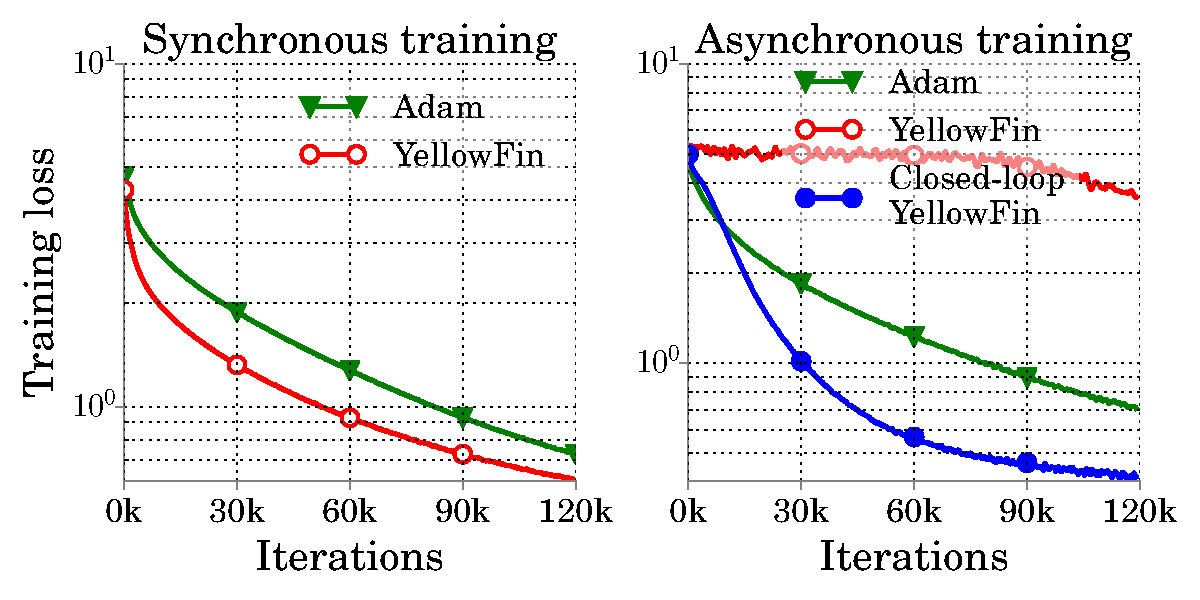
\includegraphics[width=1.0\linewidth]{experiment_results/spotlight.pdf}
	\caption{\tuner in comparison to Adam.}
\end{figure}
\end{minipage}
\end{wrapfigure}
We revisit the simple momentum SGD algorithm and propose \tuner, an automatic tuner for its hyperparameters.
A key component of \tuner is principled momentum-tuning in both synchronous and asynchronous settings.
\tuner is competitive or better that state-of-the-art adaptive methods and is asynchrony-aware by using a novel design based on measuring the level of momentum on the fly and using a closed-loop control module for momentum.

\outline{[OUR RESULTS]}
We demonstrate experimentally, in Section~\ref{sec:experiments}, that
for a large class of networks, hand-tuned momentum SGD is competitive with Adam ($0.88-1.82\times$), even though it uses fixed hyperparameters throughout execution.
On ResNets, momentum SGD can achieve a $1.25-1.82\times$ speedup over Adam.
\tuner is competitive with, and sometimes better, than state-of-the-art adaptive methods. The speedup is over $2\times$ on ResNets and $1.18\times$ on LSTMs.
Other adaptive algorithms do not tune their momentum parameter and suffer, as a result, in asynchronous settings.
Hand-tuning momentum for Adam can improve its convergence rate by up to $2\times$, when using $16$ asynchronous workers. 
Finally, closing the momentum loop in \tuner yields a speedup of $1.3-3\times$, when using $16$ asynchronous workers.
Closed-loop \tuner achieves a speedup of about $2.7\times$ over Adam on 16 asynchronous workers.

